\section{Introduction}
\label{sec:introduction}

% state the learning objective 
The objective of this laboratory assignment is to study a circuit containing 4 independent meshes and a total of 11 branches: an independent voltage source $V_A$, an independent current source $I_D$, a dependent current source $I_B$, a dependent voltage source $V_C$ and 7 resistances, from $R_1$ through to $R_7$. The circuit can be seen in Figure~\ref{fig:rc}.

In Section~\ref{sec:analysis}, a theoretical analysis of the circuit is
presented. In Section~\ref{sec:simulation}, the circuit is analysed by
simulation, and the results are compared to the theoretical results obtained in
Section~\ref{sec:analysis}. The conclusions of this study are outlined in
Section~\ref{sec:conclusion}.

\begin{figure}[h] \centering
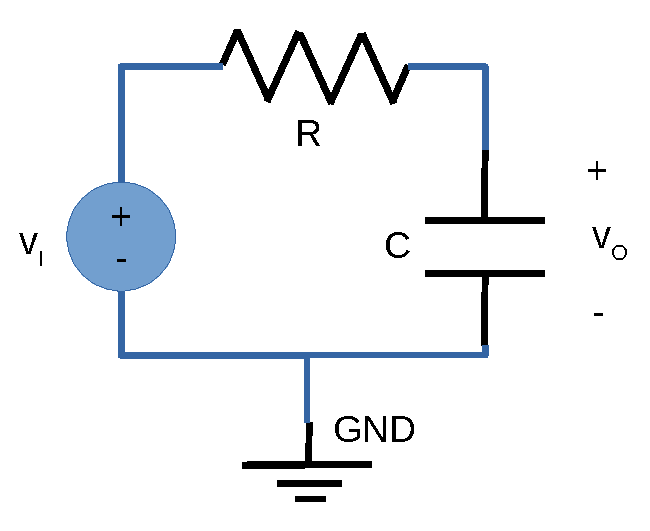
\includegraphics[width=0.9\linewidth]{rc.pdf}
\caption{Circuit with linear components.}
\label{fig:rc}
\end{figure}

